% 	HTML5 Robot User Interface Project Report: Project Planning
% 	An ASLab Project,
% 	Developed by Daniel Peiró
% 	ETSII, UPM 2014-2015
\chapter{Project Planning} \label{planning}
The development model applied to the project is a slight variation on the traditional \textit{Waterfall} model, used in many 
if not all facets of engineering. The main modification is to add an iterative loop between the Implementation phase and the 
Verification phase. This is due to the modular nature of the application that requires that each module be developed and 
tested individually, hence the loop. The reasons for the modular nature of HRUI are explained in section 
\ref{modularfrontendarchitecture}. Although this alteration may seem initially like a delay or added work, in detriment of 
the chosen modular architecture, it's actually an improvement in the efficiency of the original model. The original model's 
main problem is precisely that there are no return paths to previous phases. It basically assumes that all phases are 
completed to perfection on the first iteration, which is not at all true in real life engineering. If the model is not 
amended with solutions like the one proposed here, and is followed strictly, the result is that when arriving at the latter 
stages, problems crop up that were difficult to foresee at the start of the project. Since the model doesn't allow for 
iteration, it's sometimes necessary to return to early stages (requirements or design) to solve the problems, since the 
product was already finalized or close to it when the issues appeared. By making iterations on the implementation (and if 
required, although less likely and recommendable, to the design) after verification of small ``chunks'' of the product, 
issues remain isolated, which makes finding solutions for them easier, as well as cheaper.
\begin{figure}[H]
\centering
\captionsetup{justification=centering}
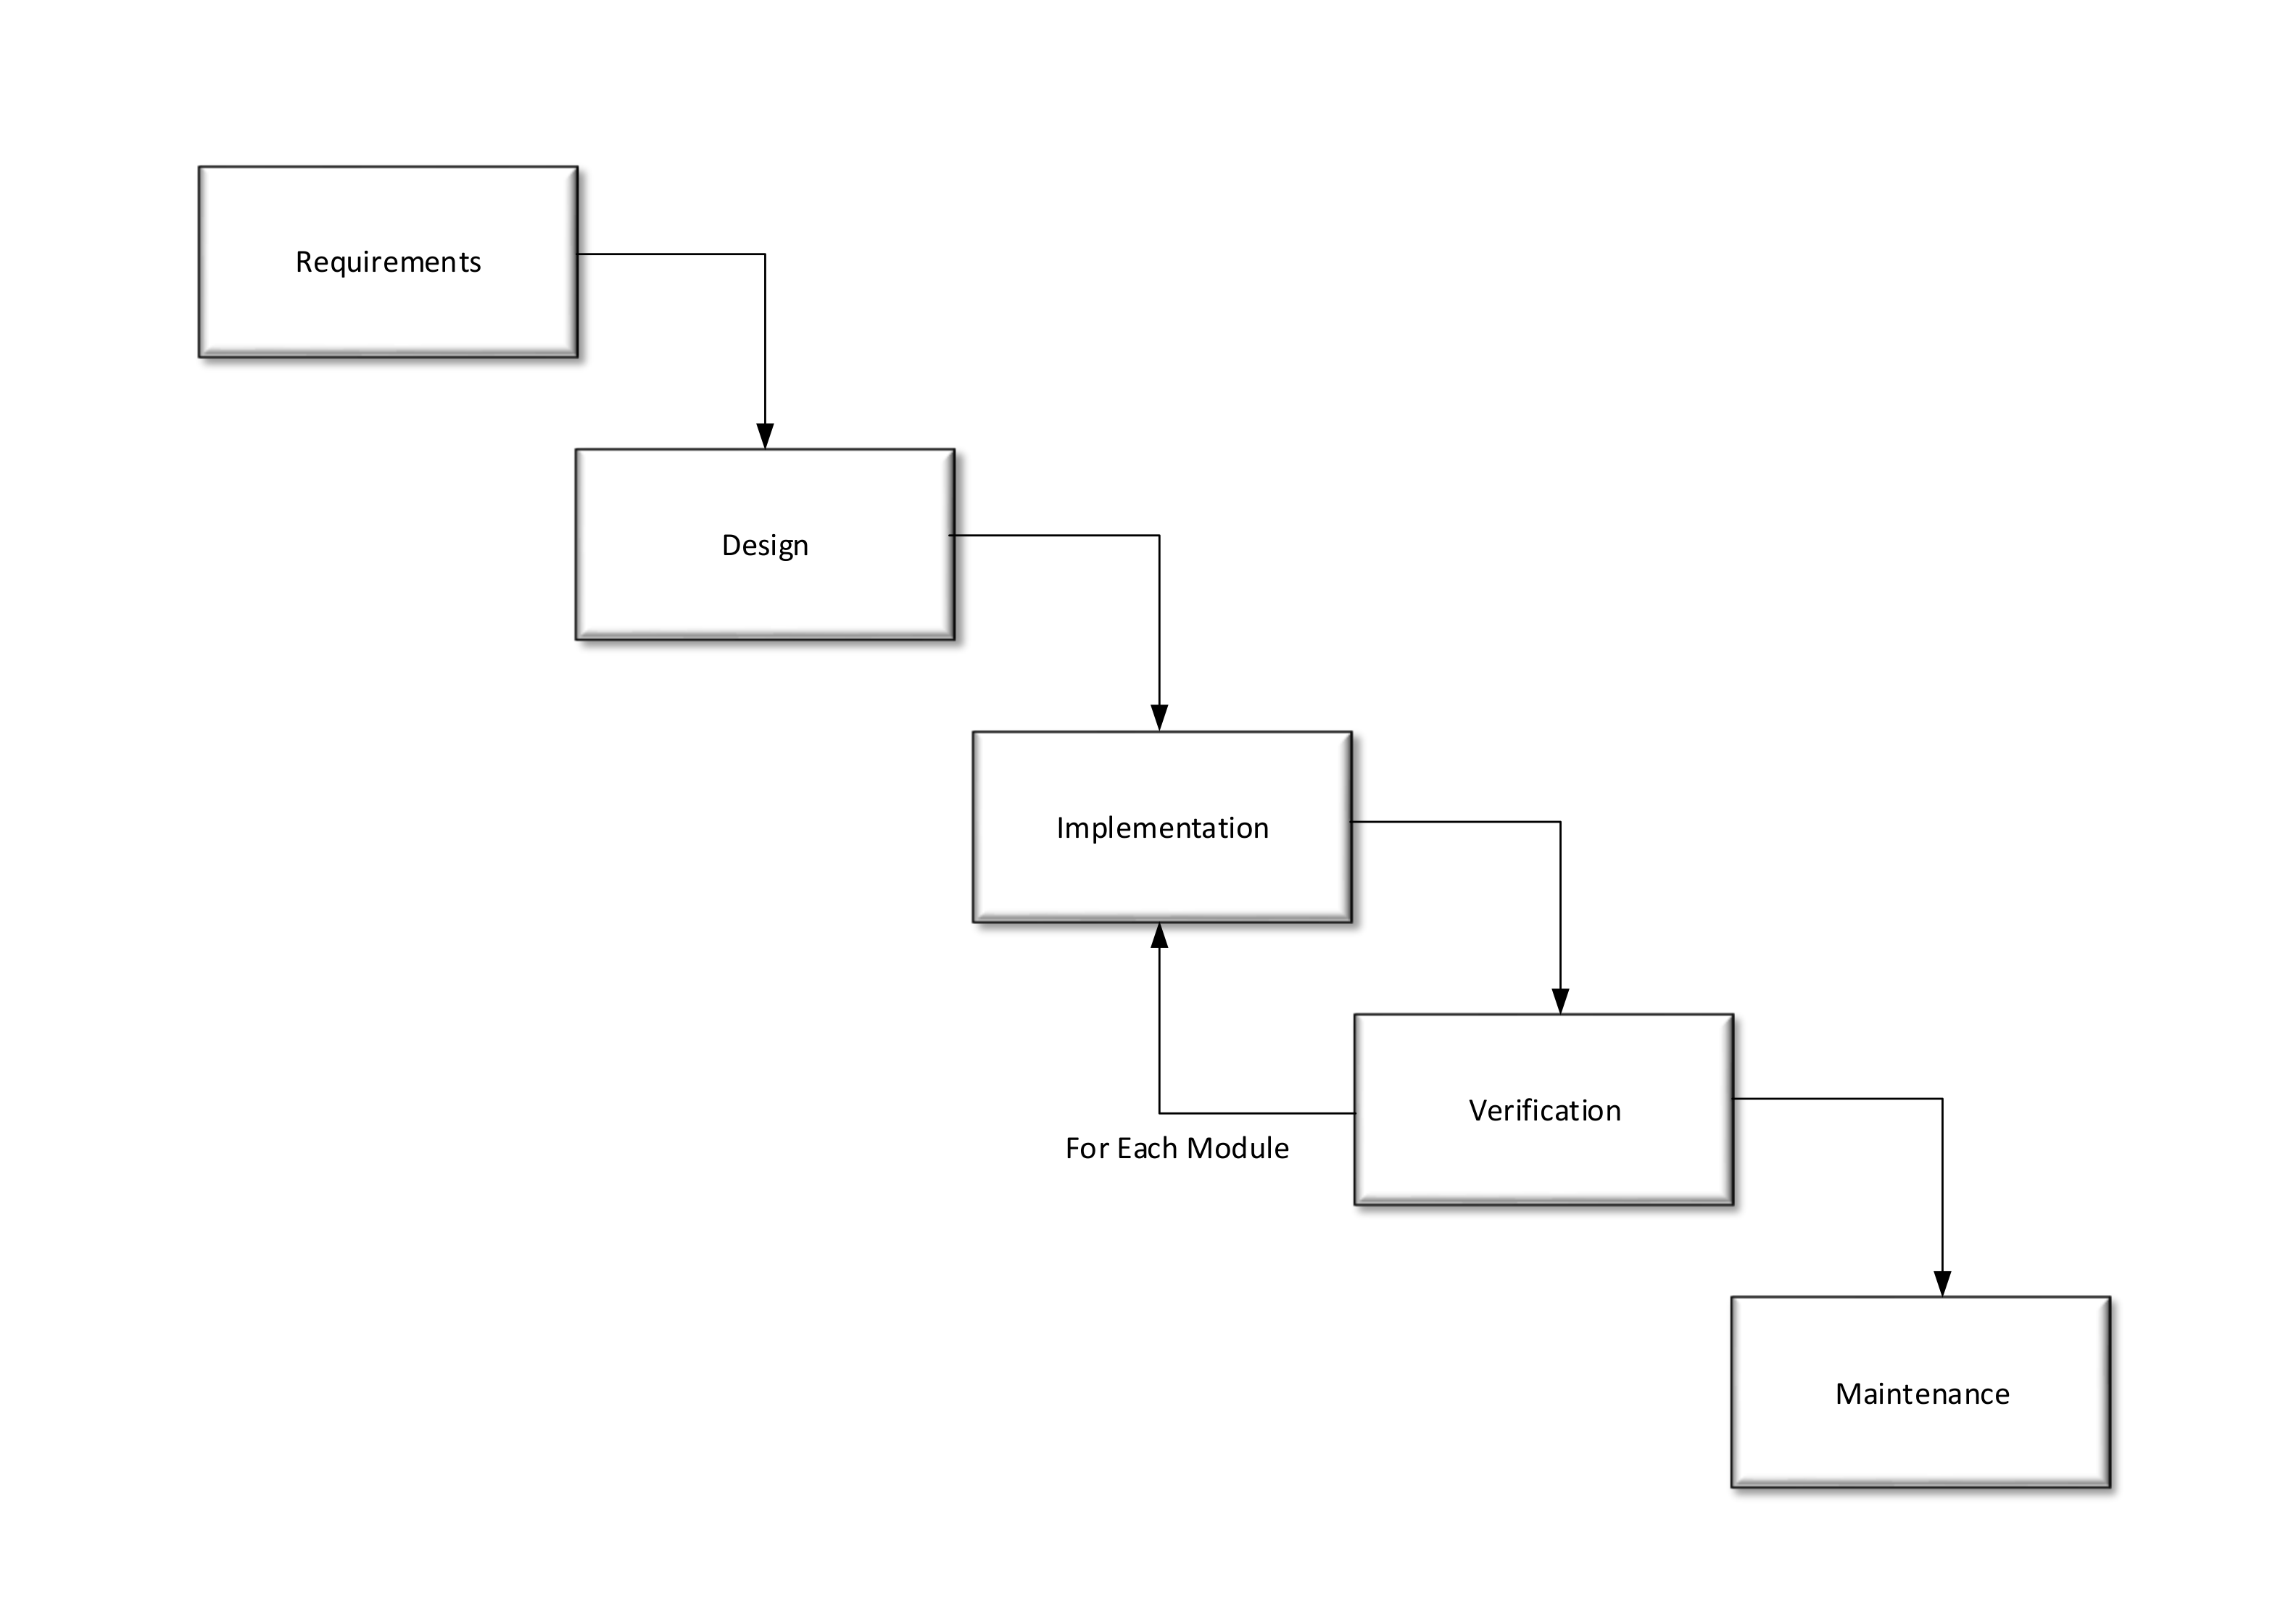
\includegraphics[width=0.7\linewidth]{waterfall}
\caption{Iterative Waterfall Development Model}
\end{figure}
\section{Work Breakdown Structure}
The following diagram shows the Work Breakdown Structure (WBS) that presents all of the deliverables in the project. It 
decomposes the project into smaller work packages that can be achieved individually, and that can be summed up to account 
for all of the work required to achieve the project's goals. The primary decomposition responds to the previously shown 
iterative waterfall development model, adding the \textit{Documentation} and \textit{Project Management} packages to the 
highest hierarchical level. The maximum level of decomposition is restricted to 4 (including the top level), for brevity.\\

Please note that in the verification package, back-end and integration testing is not explicitly included. This is 
intentional, given that the testing of the front-end modules, which are included, implicitly require testing the back-end. 
This is also true of the integrations, that are required to test the application as a whole, thus being included implicitly 
in the present packages. Testing of the back-end and the integrations cannot be considered an isolated work package, because 
testing the interface modules inherently tests these components, which cannot be utilized independently from the interface.
\begin{figure}[H]
\caption{Work Breakdown Structure (WBS) (See next page)\label{wbs}}
\end{figure}
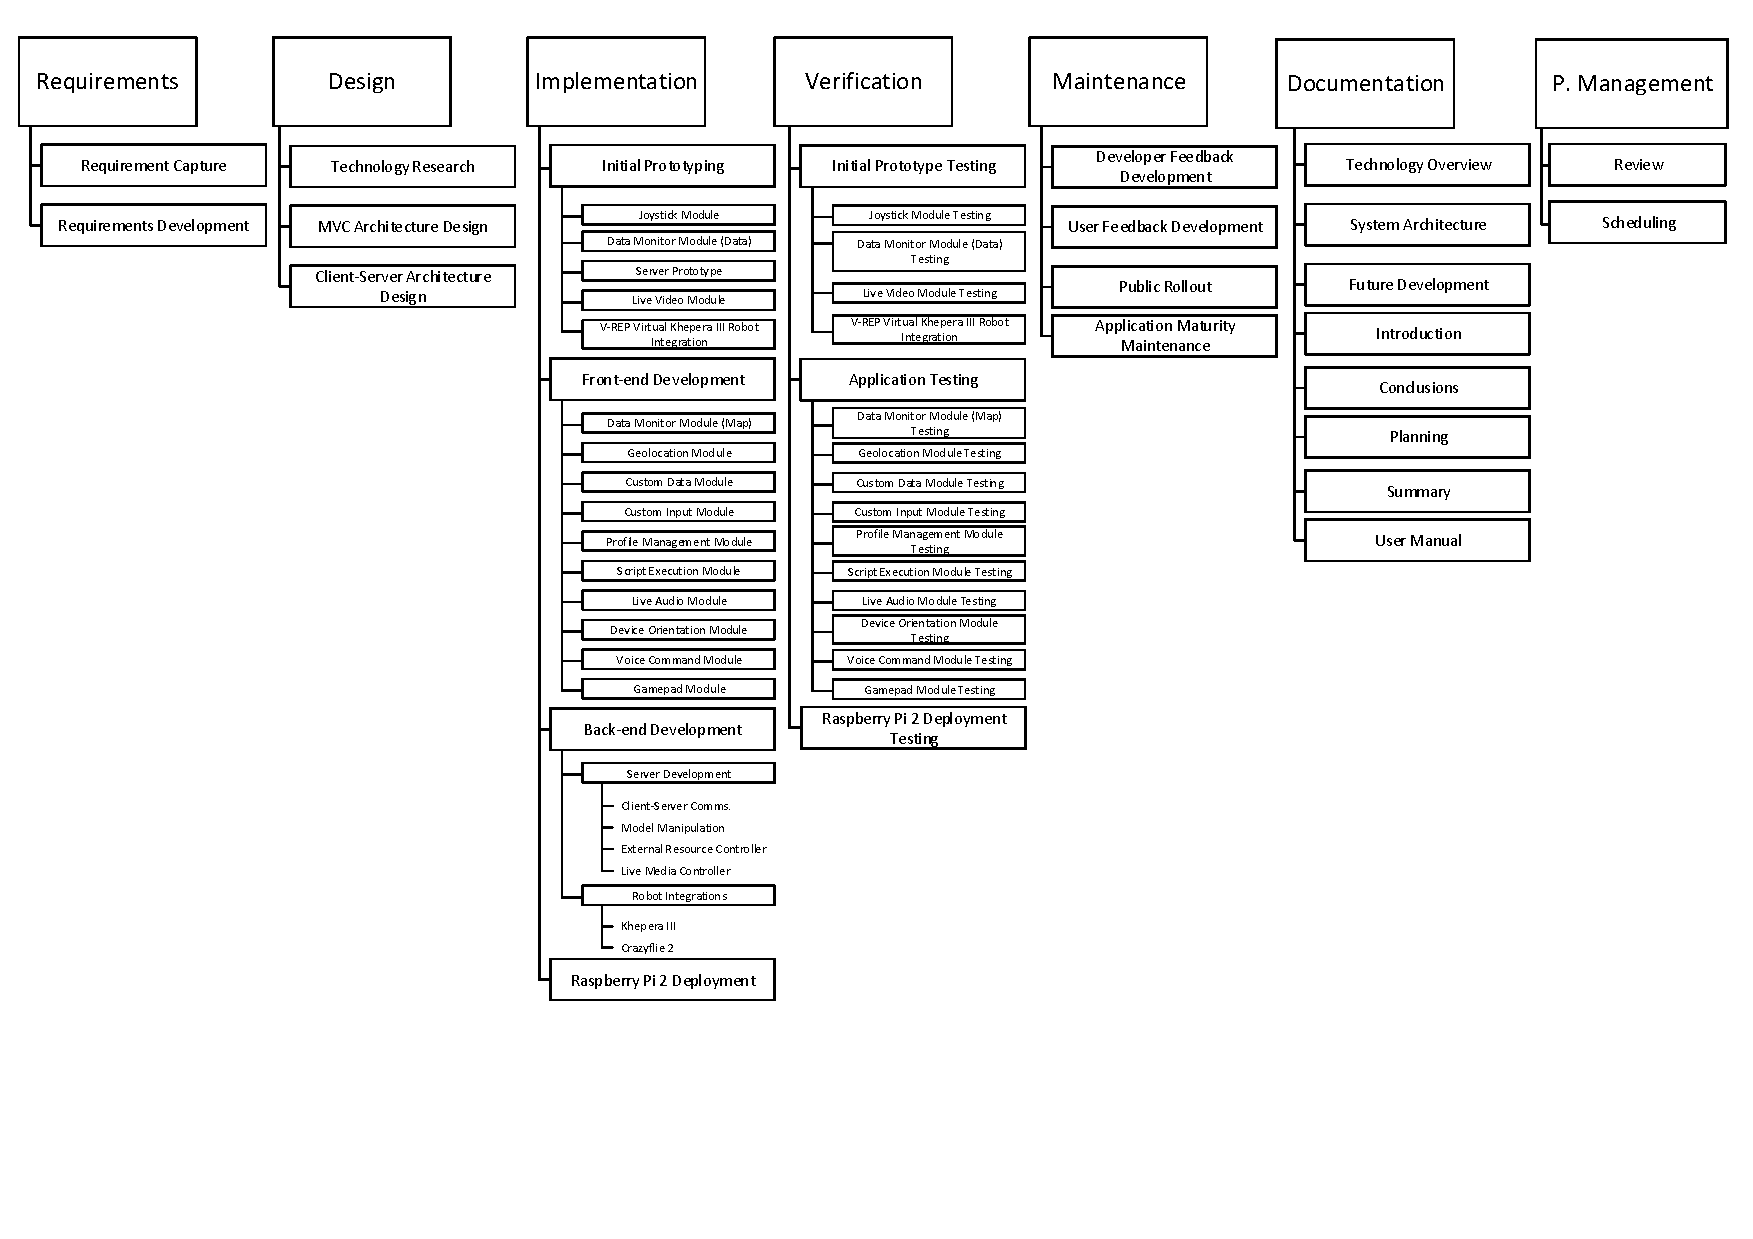
\includepdf[pages={1},landscape]{./img/wbs.pdf}
\section{Gantt Chart}
The following diagram presents the project Gantt diagram, which shows the scheduling of the project deliverables. The tasks 
are extracted directly from the Work Breakdown Structure (WBS) previously presented, while adding scheduled tasks for 
meetings.\\

Please note that there are two long periods of time where no work was scheduled for the project: October 2014 - February 
2015 and April 2015 - July 2015. This was not the initial schedule for the project, which was initially to be finished by 
March 2015. However, due to reasons unrelated to the project (the student was hired as an intern in October 2014, and is at 
the time of writing still holding the position), work on the project had to be relegated to free-time and holidays. This 
has been presented in the Gantt diagram to be accurate, even though these periods were not originally programmed. Also note 
that maintenance work is not presented in the diagram fully, given that it's a theoretical activity that would require 
several months of work, and would make the diagram too long. Regardless, maintenance planning is included in index numbers 
66 through 70, with the estimated (notice the question mark) time for fulfillment.\\

The diagram was developed using "ProjectLibre", an open-source (see section \ref{opensourcemovement}) alternative to 
Microsoft Project.
\begin{figure}[H]
\caption{Gantt Chart (See next 3 pages)\label{gantt}}
\end{figure}
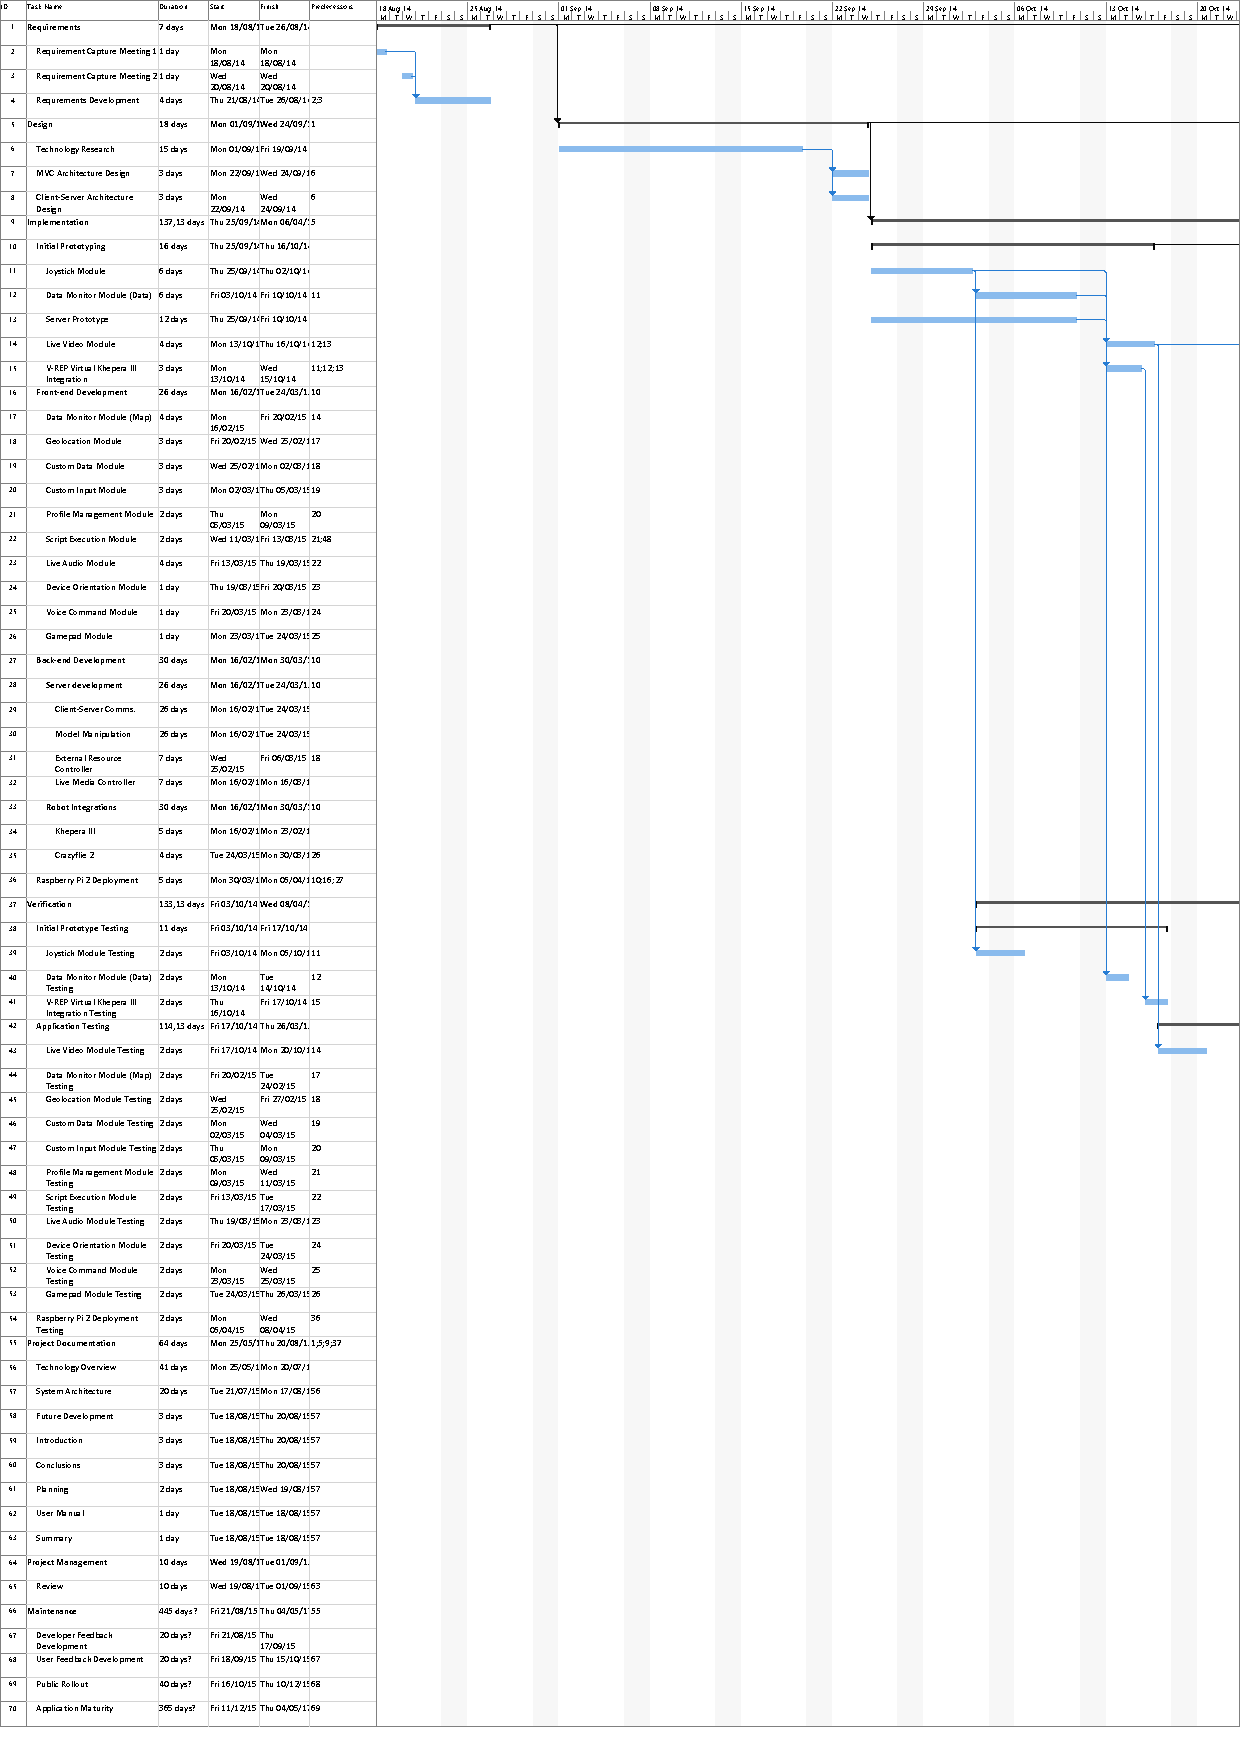
\includepdf[pages=-]{./img/gantt.pdf}
\section{Budget}
The following table details the budget for the project. The columns are:
\begin{itemize}
	\item Number (No.) : Unique identifier for each item in the budget.
	\item Concept: Brief description of the item.
	\item Quantity: The amount of the item.
	\item Units: The units in which the amount is quantified.
	\item Unitary Cost: The cost for each of the units of the item. Includes taxes unless otherwise specified.
	\item Shipping Cost: The cost associated with transport and care for the product from its manufacturing location to the 
	end user, if applicable.
	\item Total Cost: The aggregate of the shipping cost and the unitary cost times the quantity.
	\item Notes: Further item description or cost justification, if required.
\end{itemize}
The items are divided into 4 main groups:
\begin{itemize}
	\item Work: Man-hours for the project staff.
	\item Hardware: Physical objects, purchased for the project, or used mainly for the project.
	\item Software: Licenses for software used for development and report. See more on open-source licenses in section 
	\ref{opensourcemovement}.
	\item Miscellaneous.
\end{itemize}
\begin{figure}[H]
\caption{Budget (See next page)\label{budget}}
\end{figure}
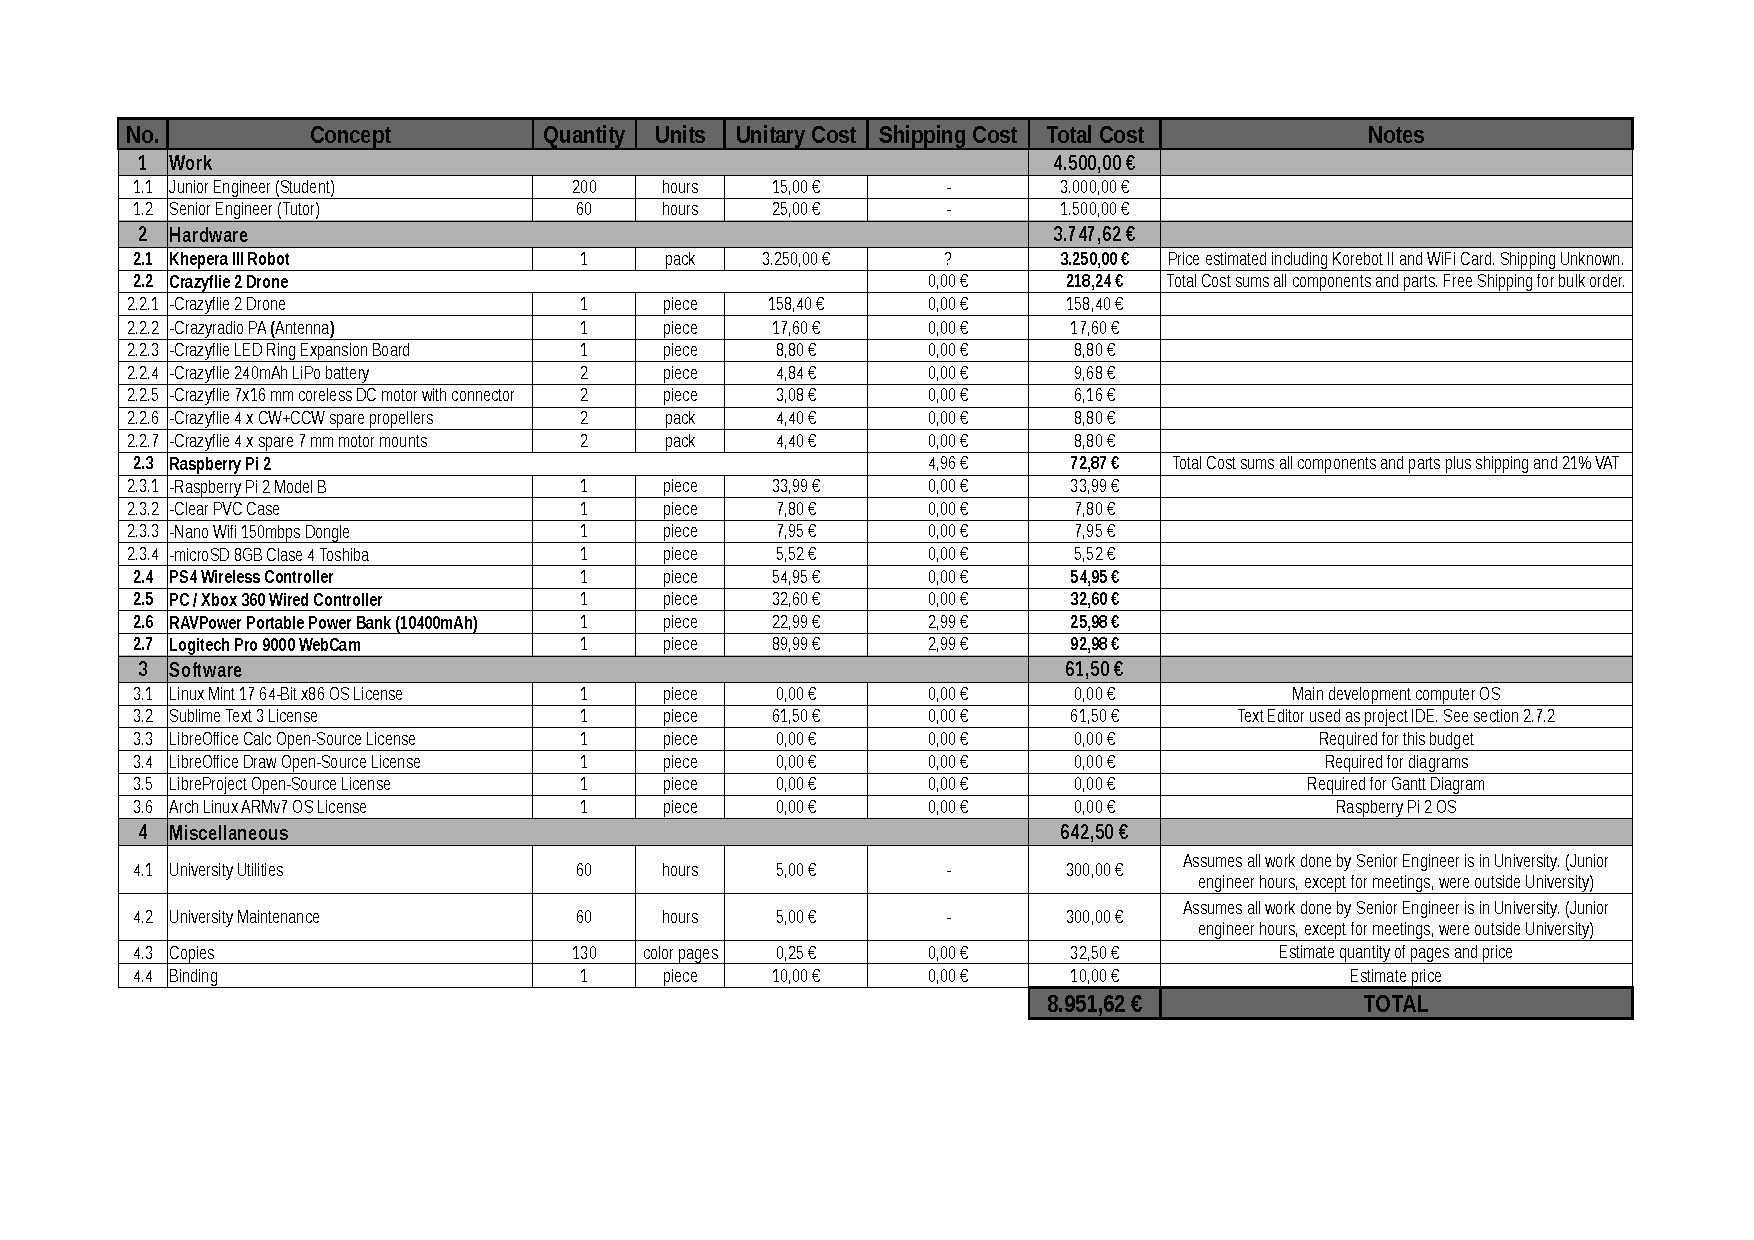
\includepdf[landscape]{./img/budget.pdf}
\section{Results}
The following figures are extracted from the GitHub graphs section for the project repository, and the report repository. 
See more on Git and GitHub in section \ref{git}. The graphs show the project time-line in the horizontal axis and the 
amount of commits made to the project repository, which is generally close to proportional to the amount of work done, in 
the vertical axis. Unfortunately, the statistics aren't necessarily an exact representation of the amount of work done, and 
therefore more sophisticated analysis, such as an S-curve or earned value management wouldn't be accurate. Nevertheless, 
these graphs provide a rough overview of the planning results of the project. It's plain to see that the majority of the 
work was done in the prototype development phase (August-October 2014), with work resuming mainly in March, and ending 
around the end of May 2015, with the addition of all the modules. There's a slight deviation from the Gantt chart in this 
second work period, where the work slips into May and part of June, although scheduled to end in April. This is mainly due 
to the addition of last minute modules like Device Orientation, Voice commands and Gamepad, which took longer than 
expected. The report graph on the other hand, stays true to the planning throughout, which is to be expected, given that 
writing the report has much more predictable challenges.\\
\begin{figure}[H]
\centering
\captionsetup{justification=centering}
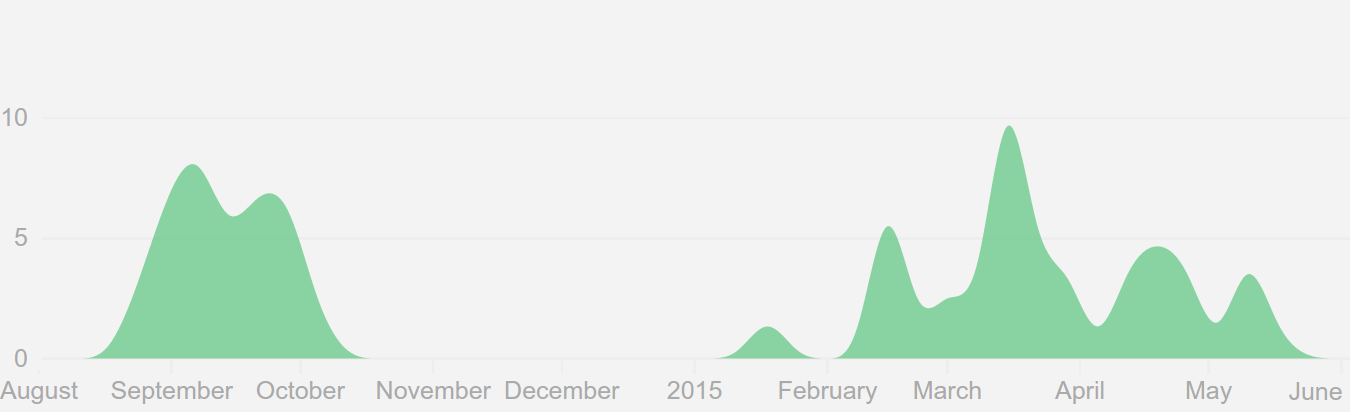
\includegraphics[width=\linewidth]{commits1}
\caption{HRUI Development Planning Results}
\end{figure}
\begin{figure}[H]
\centering
\captionsetup{justification=centering}
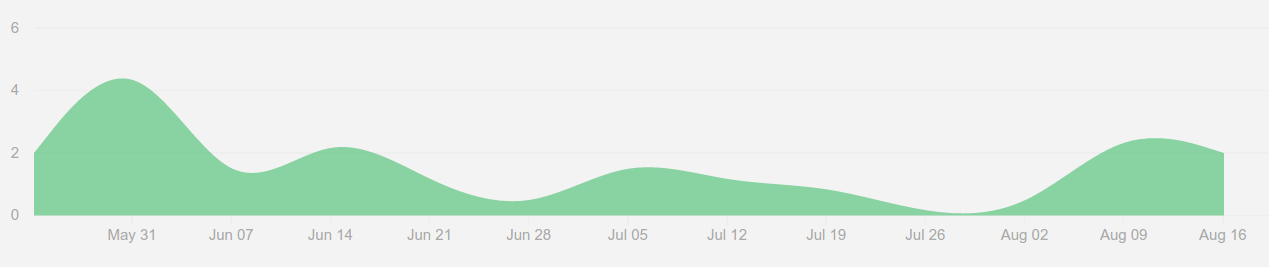
\includegraphics[width=\linewidth]{commits2}
\caption{HRUI Report Planning Results}
\end{figure}